\section{Vorlesung 5}

Zusammenfassung :\\
Folgen / Reihen / Konvergenz ? / Grenzwert ? \\ 
Neu : Funktionen\\ 
Approximation von Funktionen \\
Potenzreihen\\
Taylorreihen\\
fourierreihen\\
Näherungsweise Berechnung
\begin{definition}
$ f : \mathbb{D} \rightarrow \mathbb{R} $
heißt reelle Funktion in einer reellen veränderlichen  

\end{definition}

\begin{remark}[Definitionsbereich]
Bild von $f$ \[ f(D)= \{ f(x) \quad | \quad x \in D \} \] \\
Graph von $f$ \[ Graph(f)= \{( x \quad |\quad f(x)) \quad | \quad x \in D \} \] \\

\end{remark}   
\subsection{Stetigkeit von Funktionen an einer Stelle a }
\begin{definition}
Sei $f : D \rightarrow \mathbb{R} , D \subseteq \mathbb{R} , a \in D \quad $\\
Sei $x_n$ ist eine \textbf{Folge} 
$f$ heißt in a stetig , wenn gilt :\\
$\forall (x_n) : x_n \in D$ und 
$\limNin{f(x_n)} = f(a)$ für alle Folgen $(x_n)$\\
Die Folgenglieder sollen in Definitionsbereich liegen (Die in Definitionsbereich liegen können und den Grenzwert a haben)
\end{definition}

* Ich weiß , dass $f(x_n)$ existiert $(f(x_n)\quad ex.)$\\
 Folge $f(x_n)ex.$ , soll einen Grenzwert besitzen.$\checkmark$\\
$f(\limNin{x_n})\checkmark \checkmark$

\begin{remark}
\[ \limNin {f(x_n)= f(\limNin{x_n})} \]
$\bigstar$ Grenzwertbildung und Funktion Wertberechnung sind bei stetig Funktion in der Reihenfolge vertauschbar !  
\end{remark} 

\begin{rechnen}
$$\lim_{x \to a} f(x)$$ \\
$\textbf{d.h }$ für jede Folge $x_n$ , die gegen a konvergiert , konvergiert die Folge der Funktionierte gegen $f(a)$.
\end{rechnen}

\begin{remark}
$f$ stetig in a $\Leftrightarrow$ \\
1) $f(a)$ und \\
2) $lim_{x \to a}{f(x)}$ ex. und \\
3) Grenzwert = Funktionswert 
$\lim\limits_{x \rightarrow a}{f(x)} = f(a)$ \\


\begin{tikzpicture}[scale=1.1],

\begin{axis}[xlabel=$x$,
ylabel= $\delta$,
height=6cm,
width=10cm,
ymax=11,
ymin=0,
xmin=0,
xmax=6.5,
axis y line=left,
axis x line=bottom,
ytick={1,...,10},
yticklabels={ ,,$f(a)$ ,,},
xtick={1,...,5},
xticklabels={$x_0$,$x_2$,$a$,$x_3$,$x_1$,}
]
  \addplot[dashed] coordinates {(0,1.5) (1,1.5)};
  \addplot[dashed] coordinates {(1,0) (1,1.5)};
  \addplot[dashed] coordinates {(0,2) (2,2)};
  \addplot[dashed] coordinates {(2,0) (2,2)};
  \addplot[blue,dashed] coordinates {(0,3) (3,3)};
  \addplot[blue,dashed] coordinates {(3,0) (3,3)};
  \addplot[dashed] coordinates {(0,5) (4,5)};
  \addplot[dashed] coordinates {(4,0) (4,5)};
  \addplot[dashed] coordinates {(0,9) (5,9)};
  \addplot[dashed] coordinates {(5,0) (5,9)};

    \addplot[black,domain=1:9]  { 2^(\x-2)+1  }node {f};
    


\end{axis}
\end{tikzpicture}


\end{remark}


\begin{example}
\begin{itemize}
1)
\begin{align*}
f(x) = \frac{x^2 - 1}{x - 1} =   
\frac{(x-1)(x+1)}{(x-1)}\\ 
\end{align*}

Ist $f(x)$ stetig in $a = 1$ ?\\

a) \quad $f(1)$ ex ? nein , d.h $f$ ist in $a = 1$ nicht stetig\\ 
\\
b) $$ \lim_{x \to 1}f(x) = \lim_{x \to 1}{\frac{(x-1)(x+1)}{x-1}} = \quad ? $$

Sei $(x_n)$ eine beliebige Folge und $x_n \in D(f)$ und $\lim_{x\to \infty}(x_n)=1$
\end{itemize}
\begin{gather*}
\lim_{n \to \infty }{f(x_n)} = \lim_{n \to \infty }
{\frac{(x-1)(x+1)}{(x-1)}} = \lim_{n \to \infty }{(x_n + 1) } = \lim_{n \to \infty }{x_n} + \lim_{n \to \infty }{1} = 1 + 1 = 2 
\end{gather*}

d.h Grenzwert ex. (und es ist 2 ).
\newpage
\subsection{Verhalten bei Definitionslücken}
Bei der Annäherung der Argument von links $(x < x_0)$ bzw. von rechts $(x > x_0)$ an eine Definitionslücke $x_0$ sind folgende Fälle von besonderem Interesse:\\
(1) \textbf{hebbare Lücke bei} $x_0 = 1$\\
\begin{center}
\begin{tikzpicture}[scale=1.1],
\begin{axis}[xlabel=$x$,
ylabel= $\delta$,
height=6cm,
width=5cm,
ymax=3,
ymin=0,
xmin=0,
xmax=2,
axis y line=left,
axis x line=bottom,
ytick={1,...,10},
yticklabels={ 1,2},
xtick={1,...,5},
xticklabels={$1$}
]
    \addplot[black,domain=0:1]{x+1}node[above, sloped, pos = 0.3] {g};
    \addplot[black,domain=1:2]{x+1}node[above, sloped, pos = 0.65] {f};
    \draw [blue,  -stealth    ] (3,1) -- (1.1,2) node [right] {Lücke};
    \addplot[mark=*,fill=white] coordinates {(1,2)};

\end{axis}
\end{tikzpicture}
\end{center}

Es gilt $$\lim_{\substack{x \to x_0 \\ x < x_0}}{f(x)} = \lim_{\substack{x \to x_0 \\ x > x_0}}{f(x) = a}$$
Dann hat der Graph von $f$ an der Stelle $x_0$ lediglich ein Loch, das sich durch die Festsetzung $f(x_0) = a $ schließen lässt. Die Stelle $x_0$ heißt dann eine \textbf{herbbare Lücke} bzw. 
Man sagt , $f$ hat an der stelle 1 eine Lücke.
\end{example}

(2) $$ f(x)=\frac{1}{x} \quad ,\quad  a = 0 $$
\begin{center}
\begin{tikzpicture}[scale=1.1],
\begin{axis}[xlabel=$x$,
ylabel= $y$,
height=6cm,
width=5cm,
ymax=3,
ymin=-3,
xmin=-3,
xmax=3,
axis y line=center,
axis x line=center,
]
\addplot[domain= -3:-0.01] {1/x};
\addplot[domain= 0.01:3] {1/x};


\end{axis}
\end{tikzpicture}
\end{center}

(i) betrachte $? \lim\limits_{x \rightarrow 0^-} {f(x):}$ d.h wir
betrachten alle Folgen $(x_n)$ \\


\begin{align*}
X_n \in D , X_n \leq 0 \limNin (x_n) = 0 \\
\limNin f(x_n) = \limNin \frac{1}{x_n} \\
= \frac{\limNin {1}}{\lim\limits_{n \rightarrow - \infty}{x_n}} 
= \frac{1}{ \lim\limits_{n \rightarrow - \infty}{x_n}} = - \infty\\
\\
\text{d.h} \quad \lim_{x \to 0^-}{f(x)} \text{ex .nicht}
\end{align*}
\\
(ii) Betrachte $\lim\limits_{n \rightarrow + 0}{f(x_n)}$ , ex .nicht\\
(3)\\
\begin{center}
\begin{tikzpicture}[scale=1.1],
\begin{axis}[xlabel=$x$,
ylabel= $y$,
height=6cm,
width=5cm,
ymax=3,
ymin=-3,
xmin=-3,
xmax=3,
axis y line=center,
axis x line=center,
]
\addplot[domain= -3:-0.01] {1/x};
\addplot[domain= 0.01:3] {1};
\end{axis}
\end{tikzpicture}
\end{center}
$$
f(x) = \left\{\begin{array}{lr}
        1 , & x \geq 0\\
        \frac{1}{x} , & x < 0 
        \end{array}\right\} a = 0 \quad , \quad f(0) = 1 \quad \text{ex.}  
$$

$$ \lim\limits_{x \rightarrow 0^+}{f(x)} = 1 , 
\lim\limits_{x \rightarrow  0^-}{f(x)}= - \infty \quad \text{ex. nicht} $$
\newpage 
(4) \textbf{Sprungstelle}\\
\begin{center}
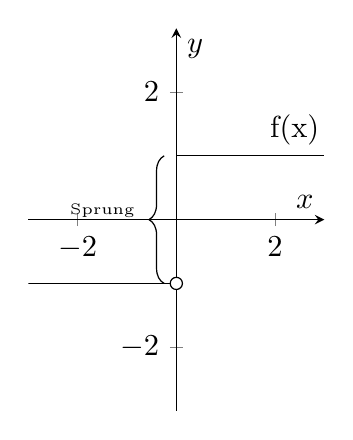
\begin{tikzpicture}[scale=1.1],
\begin{axis}[xlabel=$x$,
ylabel= $y$,
height=6cm,
width=5cm,
ymax=3,
ymin=-3,
xmin=-3,
xmax=3,
axis y line=center,
axis x line=center,
]
\addplot[domain= -3:0] {-1};
\addplot[domain= 0:3] {1} node[above ,pos=0.8] {f(x)};
\addplot[mark=*,fill=white] coordinates {(0,-1)};
  \draw [decorate, decoration={brace,amplitude=5pt,raise=4pt,mirror}] (0,1) -- (0,-1) 
node [midway, xshift=-0.5mm, yshift=1mm,auto, swap, outer sep=9pt,font=\tiny]{Sprung};
\end{axis}
\end{tikzpicture}
\end{center}
Es gilt 
$$\lim_{\substack{x \to x_0 \\ x < x_0}}{f(x)= a}$$ 
und 
$$\lim_{\substack{x \to x_0 \\ x > x_0}}{f(x)= b}$$
mit $a \neq b$
Dann hat der Graph von $f$ an der stelle $x_0$ eine \textbf{Sprungstelle}


\begin{definition}[ sgn(x)]
Die Vorzeichenfunktion oder \textbf{Signumfunktion} (von lateinisch signum ‚Zeichen‘) ist in der Mathematik eine Funktion, die einer reellen oder komplexen Zahl ihr Vorzeichen zuordnet.\\
Die reelle Signumfunktion bildet von der Menge der reellen Zahlen in die Menge \{-1,0,1\} ab und wird in der Regel wie folgt definiert:
$$ f(x) = \underbrace{sgn(x)}_{sprung}  =  \left\{\begin{array}{lr}
+ 1 , & x \geq 0\\
0 , & x = 0 \\
-1 , & x < 0 
        \end{array}\right\}$$ 
\end{definition}
$$
\neq \left\{\begin{array}{lr}
  \lim\limits_{x \rightarrow 0^-}{f(x)} = -1 \quad \text{ex.} \\
        \lim\limits_{x \rightarrow 0^+}{f(x)} = 1 \quad \text{ex.} 
        \end{array}\right\} \lim\limits_{x \rightarrow 0}{f(x)} \quad \text{ex. nicht , O heißt Sprungstelle}
$$  
\newpage
\begin{definition}
\begin{align*}
f : \rightarrow \mathbb{R} , \quad D \subseteq \mathbb{R} \quad \text{heißt \textbf{stetig} , wenn f für alle } a \in D \quad \textbf{stetig} 
\end{align*}
\end{definition}
\begin{example}
elementare Funktionen und deren Verfügungen sind stetig auf dem gesamten Definitionsbereich. \\
$\textbf{Z.B}$ \\
Polynomfunktion , rationale Funktionen, Winkelfunktionen , Potenzfunktionen , Wurzelfunktionen , Exponentialfunktionen und Logarithmusfunktion.
     
\end{example}

\begin{example}
%fehlende Skizze 
\begin{align*}
f : D \rightarrow \mathbb{R} : x \rightarrow \frac{1}{x} = x^{-1} \text{ist stetig auf dem gesamten  Defintionsbereich } D = \mathbb{R}   \backslash \{0\}  
\end{align*}

\begin{tikzpicture}[scale=1],

\begin{axis}[xlabel=$x$,
ylabel= $y$,
height=12cm,
width=17.5cm,
ymax=5,
ymin=-3,
xmin=-3,
xmax=3,
axis y line=center,
axis x line=center,
]
\addplot[domain= -3:-0.01] {1/x};
\addplot[domain= 0.01:3] {1/x};
\draw [red,  -stealth    ] (-0.5,0.7) -- (-0.1,0.1) node [left,pos=0] {kein intervall im  Definition Bereich};
\addplot[mark=*,fill=white] coordinates {(0,0)};
\addplot[ very thick,mark options={solid},blue,domain= 0.8:2.3] {1/x};
\addplot[ very thick,mark options={solid},blue,domain= 0.8:2.3] {0};
\draw [blue,  -stealth    ] (0.5,-2) -- (1.2,-0.6) node [below,pos=0] { intervall };

\end{axis}
\end{tikzpicture}

\end{example}
\newpage
\begin{beweis}
Sei $ a \in D = \mathbb{R} \backslash \{0 \}$ (d.h a $\neq 0$) 
\begin{align*}
f(a)  &= \frac{1}{a} \tag{1} \\ 
\lim_{n \to \infty}{f(x)}  &=
\lim_{n \to \infty}{\frac{1}{x}} \tag{2}
\end{align*} 

\begin{align*}
\text{Sei} \quad x_n \quad \text{eine beliebige Folge und }\quad x_n \in \underbrace{D}_{\mathbb{R}\backslash \{ 0 \}}  \quad \text{und}\quad \lim_{n \to \infty}{x_n}= a
\end{align*}
\begin{align*}
\lim_{n \to \infty}{f(x_n)}
&=  \lim_{n \to \infty}{\frac{1}{x_1}} \\
&= \frac{\lim\limits_{n \rightarrow \infty}{1}}{\lim\limits_{n \rightarrow \infty}{x_2}} \\
&= \frac{1}{a} \in \mathbb{R} \quad \text{ex.}
\end{align*}
\end{beweis}  
\subsection{Rechnenregln für Funktionen (GWS anwenden)}
%fehlende Skizze 
\begin{gather*} 
\lim\limits_{x \rightarrow \infty}{(f(x) \pm g(x))} =\lim\limits_{x \rightarrow \infty}{f(x)} \pm  \lim\limits_{x \rightarrow \infty}{g(x)} , \text{ wo bei } g(x)\neq 0  \\
\lim\limits_{n \rightarrow \infty}{(f(n) \pm g(n))} =\lim\limits_{n \rightarrow \infty}{f(n)} \pm  \lim\limits_{n \rightarrow \infty}{g(n)} 
\end{gather*}


\begin{theorem}
\begin{gather}
f: D \Rightarrow \mathbb{R} , \quad D \subseteq \mathbb{R} \text{ ist in } a \in D \text{ Stetig }
\Leftrightarrow \forall_{\epsilon} > 0 \quad \exists \delta > 0 : |x-a| < \delta \Rightarrow |f(x)- f(a)|< \epsilon 
\end{gather} 
\end{theorem}
%fehlende Skizze
  
\begin{tikzpicture}[scale=1.2],

\begin{axis}[
height=6cm,
width=10cm,
ymax=11,
ymin=0,
xmin=0,
xmax=6.5,
axis y line=left,
axis x line=bottom,
ytick={1,...,10},
yticklabels={ ,$f(a)-\epsilon$ ,,,,$f(x)$,,,$f(a)+\epsilon$},
xtick={1,...,5},
xticklabels={,,$a-\delta$,$a$,$a+\delta$}
]
\addplot[dashed] coordinates {(0,2) (2,2)};
\addplot[dashed] coordinates {(2,0) (2,2)};
\addplot[blue,dashed] coordinates {(0,3) (3,3)};
\addplot[blue,dashed] coordinates {(3,0) (3,3)};
\addplot[dashed] coordinates {(0,5) (4,5)};
\addplot[dashed] coordinates {(4,0) (4,5)};
\addplot[blue,dashed] coordinates {(0,9) (5,9)};
\addplot[blue,dashed] coordinates {(5,0) (5,9)};

\addplot[black,domain=1:9,name path=A]  { 2^(\x-2)+1  } node at (5.5, 8.5) {f};
\addplot[very thick,blue,name path=B,domain= 3:5] {0};
\addplot[blue,very thick] coordinates {(0,3) (0,9)};
\addplot[gray, pattern=north west lines] fill between[of=A and B, soft clip={domain=3:5}];
\legend{$qeg \; \epsilon$, $gce \; \delta$}
\end{axis}
\end{tikzpicture}